\section{Drift Chamber Utilities: Gas, Low Voltage and High Voltage Systems}

\subsection{Gas System: Mixing, Monitoring and Pressure Control}

The chambers operate on a gas mixture consisting of 90\% Argon and 10\% CO$_2$.
Using precision Mass-Flow Controllers (MFC), the gas is mixed and temporarily
stored in large-volume buffer tanks.  From these tanks it is delivered
to experimental Hall B.  

Argon is supplied via boil-off from a large, permanent Dewar and CO2 is supplied 
via boil-off from several standard industry high-pressure Dewars.  Two identical mixing
systems are used to mix the gas to 90\% Argon and 10\% CO$_2$ by mass using regulators and MKS G250 
mass flow controllers (MFC).  The mixed gas is then stored at ~100psig in four large-volume 
ASME pressure vessels, also called buffer tanks. This large volume smooths out 
any minor fluctuations in the Argon/CO2 ratio. To control the gas ratio, the thermal 
conductivity of the gas ratio is continually measured using Panametrics Thermal 
Conductivity Units (TCUs) and then matched to the thermal conductivity of a mixed 
gas calibration standard. Individual MFC flows are adjusted as needed if the gas mixture
ratio changes. The mixed gas is supplied to the hall via two similar gas delivery systems, 
one for R3 and one for the combined flow through R1 and R2. 

MFCs and pressure regulators set the gas flow and pressure from the 
buffer tanks to the supply manifolds in the hall. In the hall, flow control for each 
individual sector is set using rotameters located at the supply manifolds. The gas flows 
into each detector at the nose and exits out of the back-plate and into the exhaust 
manifolds. Since the gas volumes of R1 + R2 = gas volume of R3, R1 and R2 exhaust 
through the same manifold and R3 exhausts through its own manifold. The exhaust manifolds 
are connected to pressure relief systems. 

The Drift Chambers use thin, aluminized Mylar windows with a large surface area.  
Any over-pressure event could cause the windows to burst. Likewise, an under-pressure 
event could cause damage to the wires inside.  Due to the potential of catastrophic 
damage to the detectors in the case of an over-pressure or under-pressure event, 
passive relief systems (bubblers) are installed on each exhaust manifold. In an 
over-pressure situation (i.e. high differential pressure between the exhaust manifold 
and atmosphere), the gas in the detector is vented out until the differential pressure 
falls to a safe level. In an under-pressure situation (i.e. low differential pressure 
between the exhaust manifold and atmosphere), air is sucked into the exhaust manifold 
until the differential pressure increases to a safe level. Each of these high-flow 
differential pressure relief systems consist of 3 parts:  An oil filled over-pressure 
bubbler, an oil filled under-pressure bubbler, and an empty oil trap. The oil trap is 
connected to the exhaust manifold while the over and under pressure bubblers are 
connected directly to the oil trap. This prevents contaminating the exhaust manifolds
with oil. Additionally, each of the 3 parts contains baffles to remove oil droplets 
from the gas passing through the unit. 

Fig.~\ref{dc-gas-system} is a schematic of the gas delivery system 
and a snapshot 
of the control panel for monitoring the state of the system.

%%%%%%%%% Figure : dc gas system %%%%%%%%%%%%%%%%%%%%%%%%%%%%%%%%%%%%%%%%%%%%%%%
\begin{figure}[htbp]
\vspace{10cm}
\begin{picture}(50,50)
\put(-10,10)
{\hbox{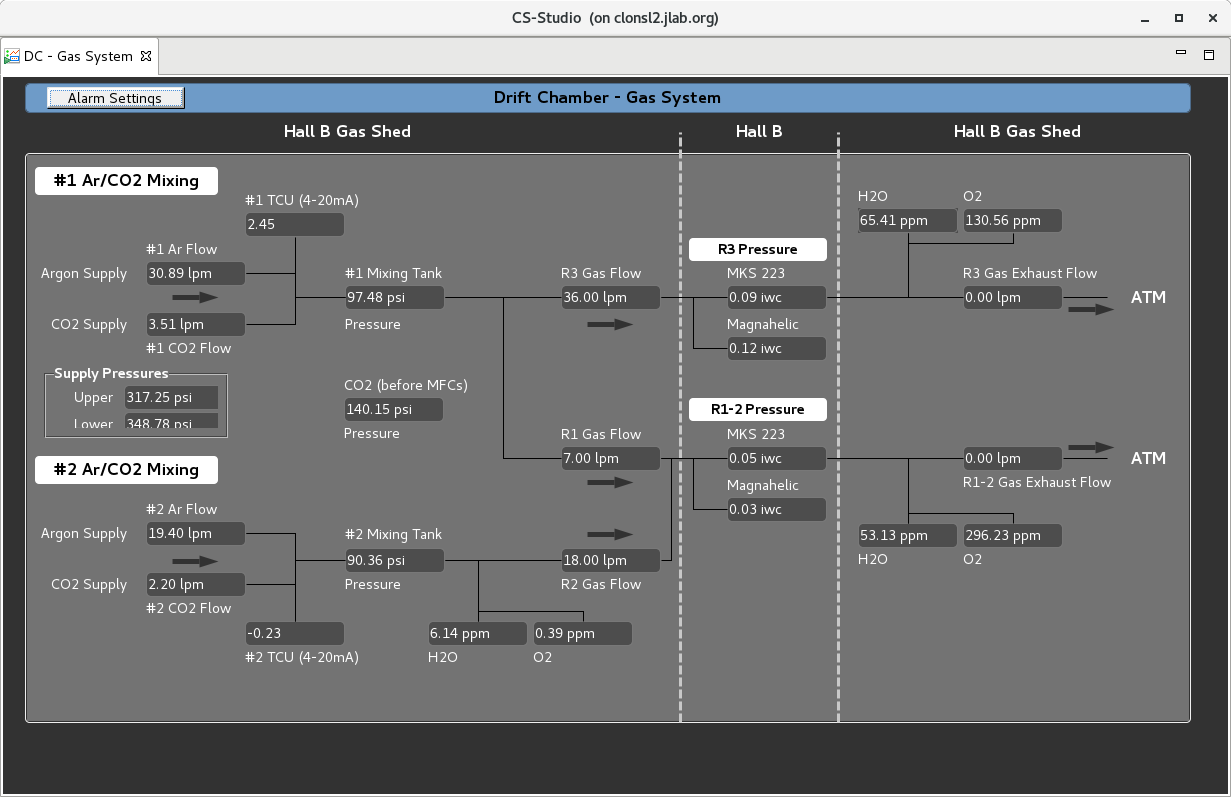
\includegraphics[width=0.8\textwidth,natwidth=610,natheight=642]{img/dc-gas-system.png}}}
\end{picture}
\caption{\small{A schematic of the drift chamber gas system showing key control and
monitoring points.}}
\label{dc-gas-system}
\end{figure}
%%%%%%%%%%%%%%%%%%%%%%%%%%%%%%%%%%%%%%%%%%%%%%%%%%%%%%%%%%%%%%%%%%%%%%%%%%%%%%%


 
\subsection{Low Voltage System}
We reused the CLAS low voltage power supplies.  
These units are robust and manufactured by Hewlett Packard.  
The supplies are remotely programmable and monitored.  The on-chamber 
pre-amplifiers require 6V and approximately 18A per chamber
(a total of 1344 pre-amps per chamber).  

We isolated the low voltage from 
ground loops by using local voltage regulators on the pre-amplifier interface 
boards (STBs).  The segmentation of the low voltage distribution cables is 
based on 32 preamplifier channels per supply cable.  Each of the supply 
cables is fused for over-current 
protection based on the average current draw of 32 pre-amplifiers.  

We designed our low voltage system: supplies, fusing, cables and control
system to be as robust and maintenance-free as possible.  To minimize
the damage to the tracking system in the event of a failure such as
a shorted pre-amplifier, we built in fine segmentation with only
32 preamplifier channels per supply cable. 
In the event of a short circuit which causes a fuse to blow,
a simple, external cable disconnect will reduce the size of the affected
area to 16 signal wires without the need to access the chambers.

Fig.~\ref{dc-lv-system} is a schematic of the low voltage
supply system and a snapshot 
of the control panel for monitoring the state of the system.
%%%%%%%%% Figure : dc low voltage system %%%%%%%%%%%%%%%%%%%%%%%%%%%%%%%%%%%%%%%%%%%%%%%
\begin{figure}[hbtp]
\vspace{10cm}
\begin{picture}(50,50)
\put(-10,10)
{\hbox{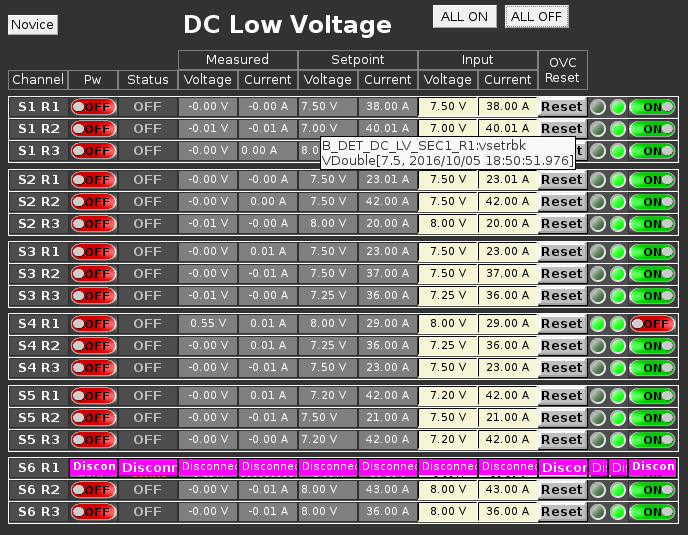
\includegraphics[width=1.2\textwidth,natwidth=610,natheight=642]{img/dc-lv-system.png}}}
\end{picture}
\caption{\small{A schematic of the low voltage control and monitoring scheme.}}
\label{dc-lv-system}
\end{figure}
%%%%%%%%%%%%%%%%%%%%%%%%%%%%%%%%%%%%%%%%%%%%%%%%%%%%%%%%%%%%%%%%%%%%%%%%%%%%%%%

\subsection{High Voltage System}

As in the case of the low-voltage system, we designed our high voltage system: 
supplies, distribution boxes, cables and control system to be as robust and 
maintenance-free as possible.  
We re-used our CAEN 
system 527 high voltage supplies with somewhat finer segmentation than our 
previous system, consistent with our total channel count dropping from 34000 
to about 24000.
To minimize the damage to the tracking system in the event of a failure such as
a broken wire, we built in very fine segmentation.
Each individual high-voltage channel powers a variable-sized group of 
wires: a 48-wire group for wires in the small-angle region, a 96-wire group
in the middle-angle region and a 192-wire group at large angles.

In the event of a failure (e.g. a broken wire) which results in a trip
of a single HV channel, we can further reduce the size of the affected
area from the whole group (48, 96 or 192 wires) to a smaller grouping
of 48 wires by an external cable disconnect without the need to 
physically access the chambers themselves.

The high-voltage supply and distribution system consists of the following:
\begin{itemize}
\item a crate-based high voltage power supply with 36 independent
high voltage channels for each drift chamber (1344 signal wires each).
Of these 36 channels, 16 supply positive high voltage to the sense
wires, 16 supply negative voltage to the field wires, and 4 supply
positive voltage to the guard wires
\item a series of two distribution boxes which distribute the high
voltage from the supply channels to variable-sized groups
of wires, with the group size being 8 wires (for small angle wires)
to 16 (intermediate angles) to 32 (large angles). 
\item  on-chamber printed circuit boards which distribute high voltage
to all of the wires; these are the HVTB's
\end{itemize}



Fig.~\ref{dc-hv-system} is a schematic of the high voltage
supply system and a snapshot 
of the control panel for monitoring the state of the system.
%%%%%%%%% Figure : dc high voltage system %%%%%%%%%%%%%%%%%%%%%%%%%%%%%%%%%%%%%%%%%%%%%%%
\begin{figure}[htbp]
\vspace{10cm}
\begin{picture}(50,50)
\put(-10,10)
{\hbox{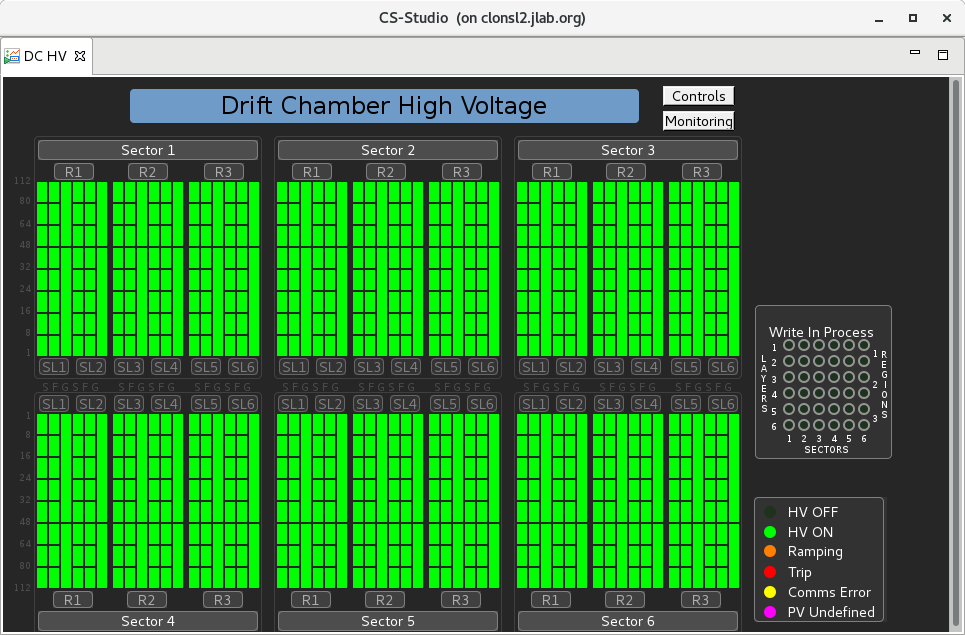
\includegraphics[width=1.\textwidth,natwidth=610,natheight=642]{img/dc-hv-system.png}}}
\end{picture}
\caption{\small{A schematic of the high voltage control and monitoring scheme, showing
the 1296 remotely controlled channels.}}
\label{dc-hv-system}
\end{figure}
%%%%%%%%%%%%%%%%%%%%%%%%%%%%%%%%%%%%%%%%%%%%%%%%%%%%%%%%%%%%%%%%%%%%%%%%%%%%%%%


